\chapter{Positron Emission Tomography (PET)}
\label{ch:pet}

% Chapter-opening illustrated modality infographic.
\begin{center}
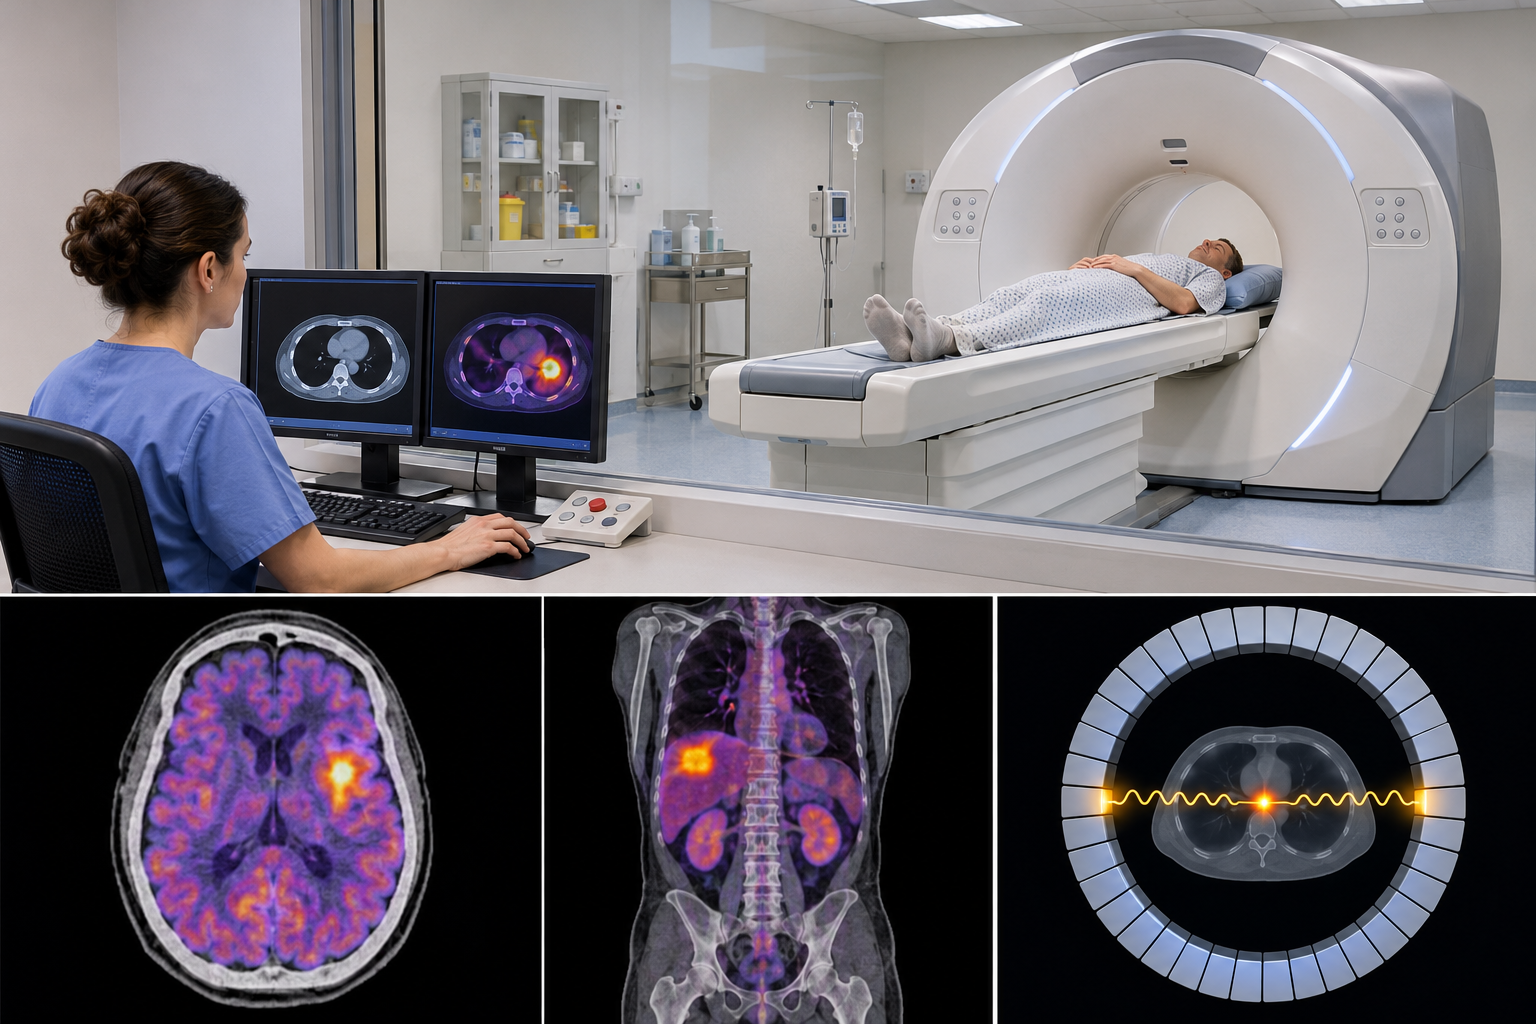
\includegraphics[width=\textwidth,keepaspectratio]{modalities/infographics/pet_realistic.png}
\end{center}
\begin{center}\footnotesize PET localizes paired annihilation photons from positron-emitting tracers to map a selected molecular process; uptake depends on the tracer. AI-generated illustration; PET images are not patient studies.\end{center}

\section{Overview}
Positron Emission Tomography (PET) is a nuclear medicine imaging modality that uses positron-emitting radiopharmaceuticals to visualize metabolic activity, tissue perfusion, molecular transport, receptor expression, and other biochemical processes within the human body.

Unlike CT and conventional MRI, PET can identify molecular and physiological abnormalities before significant anatomical changes become apparent. PET is particularly valuable for cancer staging, treatment response assessment, neurological diseases, myocardial viability, and inflammatory disorders.

This catalogue focuses specifically on PET, PET/CT, and PET/MRI, excluding SPECT and conventional scintigraphy. 

\section{Where PET is used}
The numbered entries summarize reported PET findings and radiopharmaceuticals. Findings depend on the tracer's biological target, acquisition protocol, uptake interval, reconstruction, and clinical context.

\subsection{Neurological and neurodegenerative diseases}
\begin{enumerate}[leftmargin=*,itemsep=0.45em,topsep=0.4em]
\item \textbf{Alzheimer disease.} Useful imaging findings include: Temporoparietal and posterior cingulate hypometabolism. Radiopharmaceutical: ¹⁸F-FDG.
\item \textbf{Alzheimer-associated tau pathology.} Useful imaging findings include: Increased regional tau tracer retention in adults with cognitive impairment being evaluated for Alzheimer disease. Radiopharmaceutical: ¹⁸F-Flortaucipir.
\item \textbf{Amyotrophic lateral sclerosis.} Useful imaging findings include: Altered motor cortical metabolism. Radiopharmaceutical: ¹⁸F-FDG.
\item \textbf{Cerebral amyloid pathology.} Useful imaging findings include: Increased cortical amyloid tracer retention. Radiopharmaceutical: ¹⁸F-Florbetapir.
\item \textbf{Corticobasal syndrome.} Useful imaging findings include: Asymmetric cortical and subcortical hypometabolism. Radiopharmaceutical: ¹⁸F-FDG.
\item \textbf{Creutzfeldt--Jakob disease.} Useful imaging findings include: Regional or widespread cerebral hypometabolism. Radiopharmaceutical: ¹⁸F-FDG.
\item \textbf{Dementia with Lewy bodies.} Useful imaging findings include: Occipital hypometabolism, possible cingulate island sign. Radiopharmaceutical: ¹⁸F-FDG.
\item \textbf{Frontotemporal dementia.} Useful imaging findings include: Frontal and anterior temporal hypometabolism. Radiopharmaceutical: ¹⁸F-FDG.
\item \textbf{Huntington disease.} Useful imaging findings include: Striatal hypometabolism. Radiopharmaceutical: ¹⁸F-FDG.
\item \textbf{Mild cognitive impairment.} Useful imaging findings include: Variable regional hypometabolism. Radiopharmaceutical: ¹⁸F-FDG.
\item \textbf{Multiple system atrophy.} Useful imaging findings include: Putaminal or cerebellar hypometabolism. Radiopharmaceutical: ¹⁸F-FDG.
\item \textbf{Neuroinflammatory disorders.} Useful imaging findings include: Increased tracer binding associated with neuroinflammation in research studies. Radiopharmaceutical: ¹¹C-PK11195.
\item \textbf{Parkinson disease.} Useful imaging findings include: Reduced striatal dopaminergic tracer uptake. Radiopharmaceutical: ¹⁸F-FDOPA.
\item \textbf{Posterior cortical atrophy.} Useful imaging findings include: Posterior cortical hypometabolism. Radiopharmaceutical: ¹⁸F-FDG.
\item \textbf{Primary progressive aphasia.} Useful imaging findings include: Regional language network hypometabolism. Radiopharmaceutical: ¹⁸F-FDG.
\item \textbf{Progressive supranuclear palsy.} Useful imaging findings include: Frontal, thalamic and midbrain hypometabolism. Radiopharmaceutical: ¹⁸F-FDG.
\item \textbf{Spinocerebellar ataxia.} Useful imaging findings include: Cerebellar hypometabolism. Radiopharmaceutical: ¹⁸F-FDG.
\item \textbf{Vascular dementia.} Useful imaging findings include: Multifocal regional metabolic abnormalities. Radiopharmaceutical: ¹⁸F-FDG.
\end{enumerate}

\subsection{Epilepsy}
\begin{enumerate}[leftmargin=*,itemsep=0.45em,topsep=0.4em]
\item \textbf{Drug-resistant focal epilepsy.} Useful imaging findings include: Localized or network-associated hypometabolism. Radiopharmaceutical: ¹⁸F-FDG.
\item \textbf{Focal cortical dysplasia.} Useful imaging findings include: Focal cortical metabolic abnormality. Radiopharmaceutical: ¹⁸F-FDG.
\item \textbf{Frontal lobe epilepsy.} Useful imaging findings include: Regional frontal hypometabolism. Radiopharmaceutical: ¹⁸F-FDG.
\item \textbf{Mesial temporal sclerosis.} Useful imaging findings include: Ipsilateral temporal hypometabolism. Radiopharmaceutical: ¹⁸F-FDG.
\item \textbf{MRI-negative focal epilepsy.} Useful imaging findings include: Potential localization of metabolically abnormal cortex. Radiopharmaceutical: ¹⁸F-FDG.
\item \textbf{Occipital lobe epilepsy.} Useful imaging findings include: Regional occipital hypometabolism. Radiopharmaceutical: ¹⁸F-FDG.
\item \textbf{Parietal lobe epilepsy.} Useful imaging findings include: Regional parietal hypometabolism. Radiopharmaceutical: ¹⁸F-FDG.
\item \textbf{Temporal lobe epilepsy.} Useful imaging findings include: Interictal temporal hypometabolism. Radiopharmaceutical: ¹⁸F-FDG.
\end{enumerate}

\subsection{Brain tumors}
\begin{enumerate}[leftmargin=*,itemsep=0.45em,topsep=0.4em]
\item \textbf{Astrocytoma.} Useful imaging findings include: Variable amino acid tracer uptake. Radiopharmaceutical: ¹⁸F-FET.
\item \textbf{Brain metastases.} Useful imaging findings include: Variable amino acid tracer accumulation. Radiopharmaceutical: ¹⁸F-FET.
\item \textbf{Ependymoma.} Useful imaging findings include: Variable tumor-associated tracer uptake. Radiopharmaceutical: ¹⁸F-FDG.
\item \textbf{Glioblastoma.} Useful imaging findings include: Increased amino acid transport. Radiopharmaceutical: ¹⁸F-FET.
\item \textbf{Medulloblastoma.} Useful imaging findings include: Variable increased glucose metabolism. Radiopharmaceutical: ¹⁸F-FDG.
\item \textbf{Meningioma.} Useful imaging findings include: Increased somatostatin receptor binding. Radiopharmaceutical: ⁶⁸Ga-DOTATATE.
\item \textbf{Oligodendroglioma.} Useful imaging findings include: Increased or variable amino acid uptake. Radiopharmaceutical: ¹¹C-Methionine.
\item \textbf{Primary CNS lymphoma.} Useful imaging findings include: Markedly increased glucose metabolism. Radiopharmaceutical: ¹⁸F-FDG.
\item \textbf{Radiation necrosis.} Useful imaging findings include: Frequently lower amino acid uptake than recurrent tumor, with overlap. Radiopharmaceutical: ¹⁸F-FET.
\item \textbf{Recurrent glioma.} Useful imaging findings include: Increased uptake in viable tumor tissue. Radiopharmaceutical: ¹⁸F-FET.
\item \textbf{Selected residual, recurrent, or MRI-occult pituitary adenoma.} Useful imaging findings include: Focal amino acid tracer uptake may help localize selected lesions; specialized problem-solving application. Radiopharmaceutical: ¹¹C-Methionine.
\item \textbf{Tumor pseudoprogression.} Useful imaging findings include: Variable uptake, potentially distinguishable from progression. Radiopharmaceutical: ¹⁸F-FET.
\end{enumerate}

\subsection{Cerebrovascular diseases}
\begin{enumerate}[leftmargin=*,itemsep=0.45em,topsep=0.4em]
\item \textbf{Carotid artery occlusion.} Useful imaging findings include: Abnormal cerebral perfusion and oxygen extraction. Radiopharmaceutical: ¹⁵O-Oxygen.
\item \textbf{Cerebral infarction.} Useful imaging findings include: Reduced regional glucose metabolism. Radiopharmaceutical: ¹⁸F-FDG.
\item \textbf{Cerebral ischemia.} Useful imaging findings include: Reduced regional cerebral blood flow. Radiopharmaceutical: ¹⁵O-Water.
\item \textbf{Cerebral small vessel disease.} Useful imaging findings include: Regional metabolic or perfusion abnormalities. Radiopharmaceutical: ¹⁸F-FDG.
\item \textbf{Chronic cerebral ischemia.} Useful imaging findings include: Reduced perfusion or increased oxygen extraction. Radiopharmaceutical: ¹⁵O-Water, ¹⁵O-Oxygen.
\item \textbf{Moyamoya disease.} Useful imaging findings include: Reduced cerebral perfusion reserve. Radiopharmaceutical: ¹⁵O-Water.
\end{enumerate}
These are specialized physiological assessments. PET is not a routine first-line imaging modality for acute stroke.

\subsection{Cardiovascular diseases}
\begin{enumerate}[leftmargin=*,itemsep=0.45em,topsep=0.4em]
\item \textbf{Cardiac amyloidosis (research PET).} Useful imaging findings include: Myocardial amyloid tracer retention in investigational studies; not a routine clinical PET test. Radiopharmaceutical: ¹¹C-PiB.
\item \textbf{Cardiac device infection.} Useful imaging findings include: Increased uptake surrounding implanted devices. Radiopharmaceutical: ¹⁸F-FDG.
\item \textbf{Cardiac sarcoidosis.} Useful imaging findings include: Focal or focal-on-diffuse inflammatory myocardial uptake after suppression of physiological myocardial glucose uptake. Radiopharmaceutical: ¹⁸F-FDG.
\item \textbf{Cardiac sympathetic dysfunction.} Useful imaging findings include: Altered sympathetic neuronal tracer uptake. Radiopharmaceutical: ¹¹C-HED.
\item \textbf{Coronary artery disease.} Useful imaging findings include: Stress-induced myocardial perfusion defects. Radiopharmaceutical: ⁸²Rb.
\item \textbf{Coronary microvascular dysfunction.} Useful imaging findings include: Reduced myocardial flow reserve. Radiopharmaceutical: ¹³N-Ammonia.
\item \textbf{Dilated cardiomyopathy.} Useful imaging findings include: Altered myocardial glucose metabolism; perfusion is assessed separately when indicated. Radiopharmaceutical: ¹⁸F-FDG.
\item \textbf{Hibernating myocardium.} Useful imaging findings include: Reduced perfusion with preserved glucose metabolism (perfusion--metabolism mismatch). Radiopharmaceutical: ¹⁸F-FDG with paired perfusion imaging (e.g., ⁸²Rb or ¹³N-ammonia).
\item \textbf{Hypertrophic cardiomyopathy.} Useful imaging findings include: Reduced regional myocardial flow reserve. Radiopharmaceutical: ¹³N-Ammonia.
\item \textbf{Ischemic cardiomyopathy.} Useful imaging findings include: Regional perfusion--metabolism abnormalities assessed with paired imaging. Radiopharmaceutical: ¹⁸F-FDG with a perfusion tracer (e.g., ⁸²Rb or ¹³N-ammonia).
\item \textbf{Multivessel coronary artery disease.} Useful imaging findings include: Reduced absolute myocardial blood flow. Radiopharmaceutical: ⁸²Rb.
\item \textbf{Myocardial ischemia.} Useful imaging findings include: Reversible perfusion defects. Radiopharmaceutical: ¹³N-Ammonia.
\item \textbf{Myocardial scar.} Useful imaging findings include: Matched reduction in perfusion and glucose metabolism. Radiopharmaceutical: ¹⁸F-FDG with paired perfusion imaging (e.g., ⁸²Rb or ¹³N-ammonia).
\item \textbf{Myocarditis.} Useful imaging findings include: Increased inflammatory myocardial uptake in selected cases. Radiopharmaceutical: ¹⁸F-FDG.
\item \textbf{Previous myocardial infarction.} Useful imaging findings include: Fixed perfusion defects. Radiopharmaceutical: ⁸²Rb.
\item \textbf{Prosthetic valve endocarditis.} Useful imaging findings include: Abnormal periprosthetic metabolic uptake. Radiopharmaceutical: ¹⁸F-FDG.
\end{enumerate}
Cardiac FDG studies for sarcoidosis require a dedicated preparation protocol to suppress physiological myocardial uptake; inadequate suppression can make interpretation nonspecific.

\subsection{Vascular and inflammatory arterial diseases}
\begin{enumerate}[leftmargin=*,itemsep=0.45em,topsep=0.4em]
\item \textbf{Active vascular microcalcification.} Useful imaging findings include: Increased uptake within calcifying plaques. Radiopharmaceutical: ¹⁸F-NaF.
\item \textbf{Aortitis.} Useful imaging findings include: Increased aortic wall metabolism. Radiopharmaceutical: ¹⁸F-FDG.
\item \textbf{Atherosclerosis.} Useful imaging findings include: Increased inflammatory plaque activity. Radiopharmaceutical: ¹⁸F-FDG.
\item \textbf{Giant cell arteritis.} Useful imaging findings include: Increased large arterial wall uptake. Radiopharmaceutical: ¹⁸F-FDG.
\item \textbf{Infected aortic aneurysm.} Useful imaging findings include: Increased periaortic inflammatory uptake. Radiopharmaceutical: ¹⁸F-FDG.
\item \textbf{Inflammatory abdominal aortic aneurysm.} Useful imaging findings include: Increased periaortic inflammatory activity. Radiopharmaceutical: ¹⁸F-FDG.
\item \textbf{Takayasu arteritis.} Useful imaging findings include: Increased uptake in inflamed arterial walls. Radiopharmaceutical: ¹⁸F-FDG.
\item \textbf{Vascular graft infection.} Useful imaging findings include: Abnormal graft-associated metabolic activity. Radiopharmaceutical: ¹⁸F-FDG.
\end{enumerate}
Atherosclerotic plaque characterization using PET remains predominantly investigational.

\subsection{Pulmonary and thoracic diseases}
\begin{enumerate}[leftmargin=*,itemsep=0.45em,topsep=0.4em]
\item \textbf{Bronchial carcinoid.} Useful imaging findings include: Increased somatostatin receptor uptake. Radiopharmaceutical: ⁶⁸Ga-DOTATATE.
\item \textbf{Malignant pleural mesothelioma.} Useful imaging findings include: Increased pleural metabolic uptake. Radiopharmaceutical: ¹⁸F-FDG.
\item \textbf{Mediastinal lymphadenopathy.} Useful imaging findings include: Increased nodal metabolism with malignant or inflammatory causes. Radiopharmaceutical: ¹⁸F-FDG.
\item \textbf{Non-small cell lung carcinoma.} Useful imaging findings include: Increased tumor glucose metabolism. Radiopharmaceutical: ¹⁸F-FDG.
\item \textbf{Pulmonary adenocarcinoma.} Useful imaging findings include: Variable increased metabolic activity. Radiopharmaceutical: ¹⁸F-FDG.
\item \textbf{Pulmonary fibrosis.} Useful imaging findings include: Variable uptake in affected lung tissue. Radiopharmaceutical: ¹⁸F-FDG.
\item \textbf{Pulmonary metastases.} Useful imaging findings include: Focal abnormal metabolic activity. Radiopharmaceutical: ¹⁸F-FDG.
\item \textbf{Pulmonary sarcoidosis.} Useful imaging findings include: Increased uptake in active granulomatous lesions. Radiopharmaceutical: ¹⁸F-FDG.
\item \textbf{Pulmonary squamous cell carcinoma.} Useful imaging findings include: Frequently intense glucose metabolism. Radiopharmaceutical: ¹⁸F-FDG.
\item \textbf{Pulmonary tuberculosis.} Useful imaging findings include: Increased uptake in active infectious lesions. Radiopharmaceutical: ¹⁸F-FDG.
\item \textbf{Small cell lung carcinoma.} Useful imaging findings include: Hypermetabolic primary and metastatic lesions. Radiopharmaceutical: ¹⁸F-FDG.
\item \textbf{Solitary pulmonary nodule.} Useful imaging findings include: Variable focal tracer uptake. Radiopharmaceutical: ¹⁸F-FDG.
\item \textbf{Thymic carcinoma.} Useful imaging findings include: Frequently increased glucose metabolism. Radiopharmaceutical: ¹⁸F-FDG.
\item \textbf{Thymoma.} Useful imaging findings include: Variable mediastinal metabolic activity. Radiopharmaceutical: ¹⁸F-FDG.
\end{enumerate}

\subsection{Hematological malignancies}
\begin{enumerate}[leftmargin=*,itemsep=0.45em,topsep=0.4em]
\item \textbf{Anaplastic large cell lymphoma.} Useful imaging findings include: Hypermetabolic nodal or extranodal lesions. Radiopharmaceutical: ¹⁸F-FDG.
\item \textbf{Burkitt lymphoma.} Useful imaging findings include: Markedly increased metabolic activity. Radiopharmaceutical: ¹⁸F-FDG.
\item \textbf{Diffuse large B-cell lymphoma.} Useful imaging findings include: Intense metabolic uptake. Radiopharmaceutical: ¹⁸F-FDG.
\item \textbf{Extramedullary plasmacytoma.} Useful imaging findings include: Hypermetabolic soft-tissue lesions. Radiopharmaceutical: ¹⁸F-FDG.
\item \textbf{Extranodal NK/T-cell lymphoma.} Useful imaging findings include: Increased extranodal metabolic uptake. Radiopharmaceutical: ¹⁸F-FDG.
\item \textbf{Follicular lymphoma.} Useful imaging findings include: Increased nodal metabolic activity. Radiopharmaceutical: ¹⁸F-FDG.
\item \textbf{Hodgkin lymphoma.} Useful imaging findings include: Hypermetabolic nodal and extranodal lesions. Radiopharmaceutical: ¹⁸F-FDG.
\item \textbf{Mantle cell lymphoma.} Useful imaging findings include: Variable increased metabolic uptake. Radiopharmaceutical: ¹⁸F-FDG.
\item \textbf{Marginal zone lymphoma.} Useful imaging findings include: Variable FDG avidity. Radiopharmaceutical: ¹⁸F-FDG.
\item \textbf{Multiple myeloma.} Useful imaging findings include: Metabolically active skeletal or marrow lesions. Radiopharmaceutical: ¹⁸F-FDG.
\item \textbf{Myeloid sarcoma.} Useful imaging findings include: Increased metabolic activity within extramedullary lesions. Radiopharmaceutical: ¹⁸F-FDG.
\item \textbf{Peripheral T-cell lymphoma.} Useful imaging findings include: Increased metabolic activity. Radiopharmaceutical: ¹⁸F-FDG.
\item \textbf{Primary cutaneous lymphoma.} Useful imaging findings include: Variable cutaneous metabolic uptake. Radiopharmaceutical: ¹⁸F-FDG.
\item \textbf{Primary mediastinal B-cell lymphoma.} Useful imaging findings include: Intense mediastinal metabolic activity. Radiopharmaceutical: ¹⁸F-FDG.
\item \textbf{Richter transformation.} Useful imaging findings include: Increased metabolic activity in suspicious lesions. Radiopharmaceutical: ¹⁸F-FDG.
\item \textbf{Solitary plasmacytoma.} Useful imaging findings include: Focal increased metabolic activity. Radiopharmaceutical: ¹⁸F-FDG.
\end{enumerate}

\subsection{Head and neck malignancies}
\begin{enumerate}[leftmargin=*,itemsep=0.45em,topsep=0.4em]
\item \textbf{Adenoid cystic carcinoma.} Useful imaging findings include: Variable metabolic activity. Radiopharmaceutical: ¹⁸F-FDG.
\item \textbf{Cervical nodal metastases.} Useful imaging findings include: Increased regional lymph node metabolism. Radiopharmaceutical: ¹⁸F-FDG.
\item \textbf{Esthesioneuroblastoma.} Useful imaging findings include: Increased tumor metabolism or receptor-specific uptake. Radiopharmaceutical: ¹⁸F-FDG, ⁶⁸Ga-DOTATATE.
\item \textbf{Head and neck cancer of unknown primary.} Useful imaging findings include: Potential localization of occult primary tumor. Radiopharmaceutical: ¹⁸F-FDG.
\item \textbf{Hypopharyngeal carcinoma.} Useful imaging findings include: Increased regional metabolic activity. Radiopharmaceutical: ¹⁸F-FDG.
\item \textbf{Laryngeal carcinoma.} Useful imaging findings include: Hypermetabolic laryngeal lesion. Radiopharmaceutical: ¹⁸F-FDG.
\item \textbf{Nasopharyngeal carcinoma.} Useful imaging findings include: Increased nasopharyngeal and nodal uptake. Radiopharmaceutical: ¹⁸F-FDG.
\item \textbf{Oral squamous cell carcinoma.} Useful imaging findings include: Increased tumor metabolic activity. Radiopharmaceutical: ¹⁸F-FDG.
\item \textbf{Oropharyngeal carcinoma.} Useful imaging findings include: Increased primary and nodal metabolic uptake. Radiopharmaceutical: ¹⁸F-FDG.
\item \textbf{Salivary gland carcinoma.} Useful imaging findings include: Variable tumor-associated metabolic uptake. Radiopharmaceutical: ¹⁸F-FDG.
\item \textbf{Sinonasal carcinoma.} Useful imaging findings include: Increased tumor glucose metabolism. Radiopharmaceutical: ¹⁸F-FDG.
\item \textbf{Tongue carcinoma.} Useful imaging findings include: Focal hypermetabolic lesion. Radiopharmaceutical: ¹⁸F-FDG.
\end{enumerate}

\subsection{Thyroid and parathyroid diseases}
\begin{enumerate}[leftmargin=*,itemsep=0.45em,topsep=0.4em]
\item \textbf{Anaplastic thyroid carcinoma.} Useful imaging findings include: Frequently intense glucose metabolism. Radiopharmaceutical: ¹⁸F-FDG.
\item \textbf{Ectopic parathyroid adenoma.} Useful imaging findings include: Abnormal uptake outside expected gland location. Radiopharmaceutical: ¹⁸F-Fluorocholine.
\item \textbf{Follicular thyroid carcinoma.} Useful imaging findings include: Variable metabolic activity. Radiopharmaceutical: ¹⁸F-FDG.
\item \textbf{Medullary thyroid carcinoma.} Useful imaging findings include: Increased amino acid tracer uptake. Radiopharmaceutical: ¹⁸F-FDOPA.
\item \textbf{Papillary thyroid carcinoma.} Useful imaging findings include: Increased uptake in selected non-iodine-avid lesions. Radiopharmaceutical: ¹⁸F-FDG.
\item \textbf{Parathyroid adenoma.} Useful imaging findings include: Focal fluorocholine uptake. Radiopharmaceutical: ¹⁸F-Fluorocholine.
\item \textbf{Parathyroid hyperplasia.} Useful imaging findings include: Increased uptake in hyperfunctioning glands. Radiopharmaceutical: ¹⁸F-Fluorocholine.
\item \textbf{Radioiodine-refractory thyroid carcinoma.} Useful imaging findings include: Metabolically active residual or metastatic lesions. Radiopharmaceutical: ¹⁸F-FDG.
\end{enumerate}

\subsection{Breast diseases}
\begin{enumerate}[leftmargin=*,itemsep=0.45em,topsep=0.4em]
\item \textbf{HER2-positive breast cancer.} Useful imaging findings include: Variable increased glucose metabolism. Radiopharmaceutical: ¹⁸F-FDG.
\item \textbf{Inflammatory breast cancer.} Useful imaging findings include: Diffuse breast and skin metabolic uptake. Radiopharmaceutical: ¹⁸F-FDG.
\item \textbf{Invasive ductal carcinoma.} Useful imaging findings include: Increased tumor glucose metabolism. Radiopharmaceutical: ¹⁸F-FDG.
\item \textbf{Invasive lobular carcinoma.} Useful imaging findings include: Variable or relatively low FDG uptake. Radiopharmaceutical: ¹⁸F-FDG.
\item \textbf{Metastatic breast carcinoma.} Useful imaging findings include: Abnormal uptake in metastatic sites; FES can assess estrogen receptor status in selected cases. Radiopharmaceutical: ¹⁸F-FDG; ¹⁸F-FES as an adjunct to biopsy when indicated.
\item \textbf{Recurrent breast carcinoma.} Useful imaging findings include: Increased uptake within recurrent lesions. Radiopharmaceutical: ¹⁸F-FDG.
\item \textbf{Recurrent or metastatic breast cancer with uncertain estrogen receptor status.} Useful imaging findings include: Estrogen receptor-positive lesions may be detected; FES PET is an adjunct to, not a replacement for, biopsy. Radiopharmaceutical: ¹⁸F-FES.
\item \textbf{Triple-negative breast cancer.} Useful imaging findings include: Frequently increased glucose metabolism. Radiopharmaceutical: ¹⁸F-FDG.
\end{enumerate}
PET is not a replacement for screening mammography or diagnostic breast biopsy.

\subsection{Gastrointestinal malignancies}
\begin{enumerate}[leftmargin=*,itemsep=0.45em,topsep=0.4em]
\item \textbf{Anal squamous cell carcinoma.} Useful imaging findings include: Increased primary and nodal uptake. Radiopharmaceutical: ¹⁸F-FDG.
\item \textbf{Appendiceal carcinoma.} Useful imaging findings include: Variable metabolic uptake. Radiopharmaceutical: ¹⁸F-FDG.
\item \textbf{Colorectal carcinoma.} Useful imaging findings include: Hypermetabolic primary or recurrent lesions. Radiopharmaceutical: ¹⁸F-FDG.
\item \textbf{Esophageal adenocarcinoma.} Useful imaging findings include: Increased tumor glucose metabolism. Radiopharmaceutical: ¹⁸F-FDG.
\item \textbf{Esophageal squamous cell carcinoma.} Useful imaging findings include: Frequently intense metabolic activity. Radiopharmaceutical: ¹⁸F-FDG.
\item \textbf{Gastric adenocarcinoma.} Useful imaging findings include: Variable metabolic activity. Radiopharmaceutical: ¹⁸F-FDG.
\item \textbf{Gastrointestinal lymphoma.} Useful imaging findings include: Variable or intense metabolic uptake. Radiopharmaceutical: ¹⁸F-FDG.
\item \textbf{Gastrointestinal stromal tumor.} Useful imaging findings include: Increased metabolic uptake in active tumors. Radiopharmaceutical: ¹⁸F-FDG.
\item \textbf{Peritoneal carcinomatosis.} Useful imaging findings include: Hypermetabolic peritoneal deposits. Radiopharmaceutical: ¹⁸F-FDG.
\item \textbf{Rectal carcinoma.} Useful imaging findings include: Increased uptake within viable tumor. Radiopharmaceutical: ¹⁸F-FDG.
\item \textbf{Recurrent colorectal carcinoma.} Useful imaging findings include: Increased metabolic activity at recurrence sites. Radiopharmaceutical: ¹⁸F-FDG.
\item \textbf{Small bowel adenocarcinoma.} Useful imaging findings include: Increased tumor metabolic activity. Radiopharmaceutical: ¹⁸F-FDG.
\end{enumerate}

\subsection{Liver, biliary and pancreatic malignancies}
\begin{enumerate}[leftmargin=*,itemsep=0.45em,topsep=0.4em]
\item \textbf{Extrahepatic cholangiocarcinoma.} Useful imaging findings include: Variable increased biliary tumor uptake. Radiopharmaceutical: ¹⁸F-FDG.
\item \textbf{Gallbladder carcinoma.} Useful imaging findings include: Increased tumor-associated metabolism. Radiopharmaceutical: ¹⁸F-FDG.
\item \textbf{Hepatic metastases.} Useful imaging findings include: Focal abnormal metabolic activity. Radiopharmaceutical: ¹⁸F-FDG.
\item \textbf{Hepatic neuroendocrine metastases.} Useful imaging findings include: Increased receptor-specific uptake. Radiopharmaceutical: ⁶⁸Ga-DOTATATE.
\item \textbf{Hepatocellular carcinoma.} Useful imaging findings include: Variable glucose metabolism depending on tumor differentiation. Radiopharmaceutical: ¹⁸F-FDG.
\item \textbf{Intrahepatic cholangiocarcinoma.} Useful imaging findings include: Increased metabolic uptake in many lesions. Radiopharmaceutical: ¹⁸F-FDG.
\item \textbf{Pancreatic acinar cell carcinoma.} Useful imaging findings include: Variable metabolic uptake. Radiopharmaceutical: ¹⁸F-FDG.
\item \textbf{Pancreatic ductal adenocarcinoma.} Useful imaging findings include: Increased pancreatic tumor metabolism. Radiopharmaceutical: ¹⁸F-FDG.
\item \textbf{Pancreatic neuroendocrine tumor.} Useful imaging findings include: Increased somatostatin receptor binding. Radiopharmaceutical: ⁶⁸Ga-DOTATATE.
\item \textbf{Recurrent pancreatic carcinoma.} Useful imaging findings include: Abnormal metabolic uptake at recurrence sites. Radiopharmaceutical: ¹⁸F-FDG.
\end{enumerate}

\subsection{Neuroendocrine and adrenal tumors}
\begin{enumerate}[leftmargin=*,itemsep=0.45em,topsep=0.4em]
\item \textbf{Adrenocortical carcinoma.} Useful imaging findings include: Increased glucose metabolism. Radiopharmaceutical: ¹⁸F-FDG.
\item \textbf{Bronchial carcinoid.} Useful imaging findings include: Increased somatostatin receptor tracer uptake. Radiopharmaceutical: ⁶⁸Ga-DOTATATE.
\item \textbf{Gastrinoma.} Useful imaging findings include: Increased somatostatin receptor uptake. Radiopharmaceutical: ⁶⁸Ga-DOTATATE.
\item \textbf{Gastroenteropancreatic neuroendocrine tumor.} Useful imaging findings include: Increased somatostatin receptor expression. Radiopharmaceutical: ⁶⁸Ga-DOTATATE.
\item \textbf{Glucagonoma.} Useful imaging findings include: Increased somatostatin receptor uptake. Radiopharmaceutical: ⁶⁸Ga-DOTATATE.
\item \textbf{Insulinoma.} Useful imaging findings include: Increased GLP-1 receptor tracer uptake in selected tumors. Radiopharmaceutical: ⁶⁸Ga-Exendin.
\item \textbf{Merkel cell carcinoma.} Useful imaging findings include: Increased tumor glucose metabolism. Radiopharmaceutical: ¹⁸F-FDG.
\item \textbf{Neuroblastoma.} Useful imaging findings include: Variable amino acid or glucose metabolic uptake. Radiopharmaceutical: ¹⁸F-FDOPA, ¹⁸F-FDG.
\item \textbf{Paraganglioma.} Useful imaging findings include: Frequently intense somatostatin receptor uptake. Radiopharmaceutical: ⁶⁸Ga-DOTATATE.
\item \textbf{Pheochromocytoma.} Useful imaging findings include: Increased receptor-specific or amino acid tracer uptake. Radiopharmaceutical: ⁶⁸Ga-DOTATATE, ¹⁸F-FDOPA.
\item \textbf{Poorly differentiated neuroendocrine carcinoma.} Useful imaging findings include: Frequently intense glucose metabolism. Radiopharmaceutical: ¹⁸F-FDG.
\item \textbf{Small bowel neuroendocrine tumor.} Useful imaging findings include: Receptor-positive primary and metastatic lesions. Radiopharmaceutical: ⁶⁸Ga-DOTATATE.
\item \textbf{VIPoma.} Useful imaging findings include: Increased somatostatin receptor uptake. Radiopharmaceutical: ⁶⁸Ga-DOTATATE.
\item \textbf{Well-differentiated neuroendocrine tumor.} Useful imaging findings include: Increased receptor-specific uptake. Radiopharmaceutical: ⁶⁴Cu-DOTATATE.
\end{enumerate}

\subsection{Male reproductive and urinary malignancies}
\begin{enumerate}[leftmargin=*,itemsep=0.45em,topsep=0.4em]
\item \textbf{Biochemically recurrent prostate cancer.} Useful imaging findings include: PSMA-positive recurrent or metastatic lesions. Radiopharmaceutical: ¹⁸F-DCFPyL.
\item \textbf{Bladder urothelial carcinoma.} Useful imaging findings include: Increased uptake in selected primary or metastatic lesions. Radiopharmaceutical: ¹⁸F-FDG.
\item \textbf{Metastatic castration-resistant prostate cancer.} Useful imaging findings include: Variable PSMA expression in metastatic lesions. Radiopharmaceutical: ⁶⁸Ga-PSMA-11.
\item \textbf{Neuroendocrine prostate carcinoma.} Useful imaging findings include: Increased FDG uptake with potentially reduced PSMA expression. Radiopharmaceutical: ¹⁸F-FDG.
\item \textbf{Penile squamous cell carcinoma.} Useful imaging findings include: Increased primary or metastatic uptake. Radiopharmaceutical: ¹⁸F-FDG.
\item \textbf{Prostate adenocarcinoma.} Useful imaging findings include: Increased PSMA-targeted tracer uptake. Radiopharmaceutical: ⁶⁸Ga-PSMA-11.
\item \textbf{Renal cell carcinoma.} Useful imaging findings include: Variable uptake, particularly in metastatic disease. Radiopharmaceutical: ¹⁸F-FDG.
\item \textbf{Renal lymphoma.} Useful imaging findings include: Markedly increased metabolic activity. Radiopharmaceutical: ¹⁸F-FDG.
\item \textbf{Testicular seminoma.} Useful imaging findings include: Increased uptake in selected residual tumor masses. Radiopharmaceutical: ¹⁸F-FDG.
\item \textbf{Upper urinary tract urothelial carcinoma.} Useful imaging findings include: Variable metabolic activity. Radiopharmaceutical: ¹⁸F-FDG.
\end{enumerate}

\subsection{Female reproductive malignancies}
\begin{enumerate}[leftmargin=*,itemsep=0.45em,topsep=0.4em]
\item \textbf{Cervical carcinoma.} Useful imaging findings include: Increased cervical and metastatic metabolic uptake. Radiopharmaceutical: ¹⁸F-FDG.
\item \textbf{Endometrial carcinoma.} Useful imaging findings include: Increased uterine or metastatic metabolic activity. Radiopharmaceutical: ¹⁸F-FDG.
\item \textbf{Endometrial stromal sarcoma.} Useful imaging findings include: Variable metabolic uptake. Radiopharmaceutical: ¹⁸F-FDG.
\item \textbf{Fallopian tube carcinoma.} Useful imaging findings include: Increased tumor-associated uptake. Radiopharmaceutical: ¹⁸F-FDG.
\item \textbf{Ovarian epithelial carcinoma.} Useful imaging findings include: Hypermetabolic pelvic and peritoneal lesions. Radiopharmaceutical: ¹⁸F-FDG.
\item \textbf{Primary peritoneal carcinoma.} Useful imaging findings include: Hypermetabolic peritoneal deposits. Radiopharmaceutical: ¹⁸F-FDG.
\item \textbf{Recurrent ovarian carcinoma.} Useful imaging findings include: Increased metabolic activity within recurrent lesions. Radiopharmaceutical: ¹⁸F-FDG.
\item \textbf{Uterine leiomyosarcoma.} Useful imaging findings include: Frequently increased glucose metabolism. Radiopharmaceutical: ¹⁸F-FDG.
\item \textbf{Vaginal carcinoma.} Useful imaging findings include: Increased tumor-associated metabolic activity. Radiopharmaceutical: ¹⁸F-FDG.
\item \textbf{Vulvar carcinoma.} Useful imaging findings include: Increased primary and nodal metabolic uptake. Radiopharmaceutical: ¹⁸F-FDG.
\end{enumerate}

\subsection{Bone and soft-tissue tumors}
\begin{enumerate}[leftmargin=*,itemsep=0.45em,topsep=0.4em]
\item \textbf{Angiosarcoma.} Useful imaging findings include: Variable increased metabolic uptake. Radiopharmaceutical: ¹⁸F-FDG.
\item \textbf{Bone lymphoma.} Useful imaging findings include: Markedly increased skeletal metabolic activity. Radiopharmaceutical: ¹⁸F-FDG.
\item \textbf{Chondrosarcoma.} Useful imaging findings include: Variable metabolic uptake depending on tumor grade. Radiopharmaceutical: ¹⁸F-FDG.
\item \textbf{Chordoma.} Useful imaging findings include: Variable metabolic activity. Radiopharmaceutical: ¹⁸F-FDG.
\item \textbf{Desmoid-type fibromatosis.} Useful imaging findings include: Variable metabolic activity. Radiopharmaceutical: ¹⁸F-FDG.
\item \textbf{Ewing sarcoma.} Useful imaging findings include: Frequently intense metabolic uptake. Radiopharmaceutical: ¹⁸F-FDG.
\item \textbf{Giant cell tumor of bone.} Useful imaging findings include: Frequently intense uptake despite benign or intermediate pathology. Radiopharmaceutical: ¹⁸F-FDG.
\item \textbf{Leiomyosarcoma.} Useful imaging findings include: Increased glucose metabolism in viable tumor. Radiopharmaceutical: ¹⁸F-FDG.
\item \textbf{Liposarcoma.} Useful imaging findings include: Variable uptake depending on histological subtype. Radiopharmaceutical: ¹⁸F-FDG.
\item \textbf{Malignant peripheral nerve sheath tumor.} Useful imaging findings include: Frequently increased metabolic activity. Radiopharmaceutical: ¹⁸F-FDG.
\item \textbf{Osteoblastic bone metastases.} Useful imaging findings include: Increased skeletal mineral turnover. Radiopharmaceutical: ¹⁸F-NaF.
\item \textbf{Osteolytic bone metastases.} Useful imaging findings include: Increased metabolism in viable tumor. Radiopharmaceutical: ¹⁸F-FDG.
\item \textbf{Osteosarcoma.} Useful imaging findings include: Increased tumor glucose metabolism. Radiopharmaceutical: ¹⁸F-FDG.
\item \textbf{Rhabdomyosarcoma.} Useful imaging findings include: Increased metabolic activity. Radiopharmaceutical: ¹⁸F-FDG.
\item \textbf{Synovial sarcoma.} Useful imaging findings include: Increased tumor-associated metabolic activity. Radiopharmaceutical: ¹⁸F-FDG.
\item \textbf{Undifferentiated pleomorphic sarcoma.} Useful imaging findings include: Increased tumor glucose metabolism. Radiopharmaceutical: ¹⁸F-FDG.
\end{enumerate}

\subsection{Skin malignancies}
\begin{enumerate}[leftmargin=*,itemsep=0.45em,topsep=0.4em]
\item \textbf{Cutaneous lymphoma.} Useful imaging findings include: Variable increased cutaneous metabolic uptake. Radiopharmaceutical: ¹⁸F-FDG.
\item \textbf{Cutaneous squamous cell carcinoma.} Useful imaging findings include: Increased metabolic uptake in advanced disease. Radiopharmaceutical: ¹⁸F-FDG.
\item \textbf{Dermatofibrosarcoma protuberans.} Useful imaging findings include: Variable tumor metabolic activity. Radiopharmaceutical: ¹⁸F-FDG.
\item \textbf{Malignant melanoma.} Useful imaging findings include: Hypermetabolic primary or metastatic lesions. Radiopharmaceutical: ¹⁸F-FDG.
\item \textbf{Merkel cell carcinoma.} Useful imaging findings include: Frequently intense metabolic activity. Radiopharmaceutical: ¹⁸F-FDG.
\end{enumerate}

\subsection{Infectious diseases}
\begin{enumerate}[leftmargin=*,itemsep=0.45em,topsep=0.4em]
\item \textbf{Acute osteomyelitis.} Useful imaging findings include: Increased osseous inflammatory metabolism. Radiopharmaceutical: ¹⁸F-FDG.
\item \textbf{Chronic osteomyelitis.} Useful imaging findings include: Persistent focal skeletal metabolic activity. Radiopharmaceutical: ¹⁸F-FDG.
\item \textbf{Diabetic foot osteomyelitis.} Useful imaging findings include: Increased osseous inflammatory uptake. Radiopharmaceutical: ¹⁸F-FDG.
\item \textbf{Disseminated infection.} Useful imaging findings include: Multiple abnormal inflammatory foci. Radiopharmaceutical: ¹⁸F-FDG.
\item \textbf{Fever of unknown origin.} Useful imaging findings include: Localization of abnormal metabolic foci. Radiopharmaceutical: ¹⁸F-FDG.
\item \textbf{Fungal infection.} Useful imaging findings include: Increased metabolic activity in affected tissues. Radiopharmaceutical: ¹⁸F-FDG.
\item \textbf{Hepatic abscess.} Useful imaging findings include: Increased inflammatory uptake, often peripheral. Radiopharmaceutical: ¹⁸F-FDG.
\item \textbf{Infected hepatic cyst.} Useful imaging findings include: Increased cyst-associated inflammatory uptake. Radiopharmaceutical: ¹⁸F-FDG.
\item \textbf{Infected orthopedic hardware.} Useful imaging findings include: Increased peri-implant metabolic activity. Radiopharmaceutical: ¹⁸F-FDG.
\item \textbf{Infected renal cyst.} Useful imaging findings include: Increased cyst wall metabolic activity. Radiopharmaceutical: ¹⁸F-FDG.
\item \textbf{Intra-abdominal abscess.} Useful imaging findings include: Focal inflammatory metabolic uptake. Radiopharmaceutical: ¹⁸F-FDG.
\item \textbf{Prosthetic joint infection.} Useful imaging findings include: Abnormal periprosthetic uptake, with limited specificity. Radiopharmaceutical: ¹⁸F-FDG.
\item \textbf{Septic emboli.} Useful imaging findings include: Multifocal inflammatory metabolic abnormalities. Radiopharmaceutical: ¹⁸F-FDG.
\item \textbf{Spondylodiscitis.} Useful imaging findings include: Increased uptake involving disc and adjacent vertebral structures. Radiopharmaceutical: ¹⁸F-FDG.
\item \textbf{Tuberculosis.} Useful imaging findings include: Hypermetabolic infectious lesions. Radiopharmaceutical: ¹⁸F-FDG.
\item \textbf{Vertebral osteomyelitis.} Useful imaging findings include: Increased vertebral uptake. Radiopharmaceutical: ¹⁸F-FDG.
\end{enumerate}

\subsection{Autoimmune and systemic inflammatory diseases}
\begin{enumerate}[leftmargin=*,itemsep=0.45em,topsep=0.4em]
\item \textbf{Autoimmune pancreatitis.} Useful imaging findings include: Diffuse or focal pancreatic metabolic uptake. Radiopharmaceutical: ¹⁸F-FDG.
\item \textbf{Crohn disease.} Useful imaging findings include: Increased inflammatory bowel wall metabolism. Radiopharmaceutical: ¹⁸F-FDG.
\item \textbf{Dermatomyositis.} Useful imaging findings include: Increased muscle-associated inflammatory uptake in some cases. Radiopharmaceutical: ¹⁸F-FDG.
\item \textbf{IgG4-related disease.} Useful imaging findings include: Multiorgan inflammatory metabolic uptake. Radiopharmaceutical: ¹⁸F-FDG.
\item \textbf{Polymyalgia rheumatica.} Useful imaging findings include: Characteristic periarticular inflammatory uptake. Radiopharmaceutical: ¹⁸F-FDG.
\item \textbf{Polymyositis.} Useful imaging findings include: Increased muscle metabolism in active inflammation. Radiopharmaceutical: ¹⁸F-FDG.
\item \textbf{Psoriatic arthritis.} Useful imaging findings include: Increased joint or entheseal inflammatory activity. Radiopharmaceutical: ¹⁸F-FDG.
\item \textbf{Relapsing polychondritis.} Useful imaging findings include: Increased uptake in inflamed cartilaginous structures. Radiopharmaceutical: ¹⁸F-FDG.
\item \textbf{Retroperitoneal fibrosis.} Useful imaging findings include: Increased metabolic activity in active fibrotic tissue. Radiopharmaceutical: ¹⁸F-FDG.
\item \textbf{Rheumatoid arthritis.} Useful imaging findings include: Increased synovial metabolic activity. Radiopharmaceutical: ¹⁸F-FDG.
\item \textbf{Systemic sarcoidosis.} Useful imaging findings include: Hypermetabolic granulomatous lesions. Radiopharmaceutical: ¹⁸F-FDG.
\item \textbf{Ulcerative colitis.} Useful imaging findings include: Increased colonic inflammatory uptake. Radiopharmaceutical: ¹⁸F-FDG.
\end{enumerate}

\subsection{Nonmalignant skeletal disorders}
\begin{enumerate}[leftmargin=*,itemsep=0.45em,topsep=0.4em]
\item \textbf{Aseptic prosthetic loosening.} Useful imaging findings include: Increased periprosthetic bone remodeling. Radiopharmaceutical: ¹⁸F-NaF.
\item \textbf{Fibrous dysplasia.} Useful imaging findings include: Increased skeletal remodeling activity. Radiopharmaceutical: ¹⁸F-NaF.
\item \textbf{Heterotopic ossification.} Useful imaging findings include: Increased extraosseous mineralization. Radiopharmaceutical: ¹⁸F-NaF.
\item \textbf{Insufficiency fracture.} Useful imaging findings include: Increased tracer uptake at fracture sites. Radiopharmaceutical: ¹⁸F-NaF.
\item \textbf{Osteoarthritis.} Useful imaging findings include: Increased subchondral bone turnover. Radiopharmaceutical: ¹⁸F-NaF.
\item \textbf{Osteonecrosis.} Useful imaging findings include: Variable regional skeletal tracer uptake. Radiopharmaceutical: ¹⁸F-NaF.
\item \textbf{Paget disease of bone.} Useful imaging findings include: Intense skeletal mineral turnover. Radiopharmaceutical: ¹⁸F-NaF.
\item \textbf{Stress fracture.} Useful imaging findings include: Focal increased bone remodeling. Radiopharmaceutical: ¹⁸F-NaF.
\end{enumerate}

\subsection{Summary of catalogue}
\begin{center}
\begin{tabular}{@{}p{0.70\textwidth}r@{}}
\toprule
\textbf{Disease category} & \textbf{Entries} \\
\midrule
Autoimmune and systemic inflammatory diseases & 12 \\
Bone and soft-tissue tumors & 16 \\
Brain tumors & 12 \\
Breast diseases & 8 \\
Cardiovascular diseases & 16 \\
Cerebrovascular diseases & 6 \\
Epilepsy & 8 \\
Female reproductive malignancies & 10 \\
Gastrointestinal malignancies & 12 \\
Head and neck malignancies & 12 \\
Hematological malignancies & 16 \\
Infectious diseases & 16 \\
Liver, biliary and pancreatic malignancies & 10 \\
Male reproductive and urinary malignancies & 10 \\
Neuroendocrine and adrenal tumors & 14 \\
Neurological and neurodegenerative diseases & 18 \\
Nonmalignant skeletal disorders & 8 \\
Pulmonary and thoracic diseases & 14 \\
Skin malignancies & 5 \\
Thyroid and parathyroid diseases & 8 \\
Vascular and inflammatory arterial diseases & 8 \\
\midrule
\textbf{Total} & \textbf{239} \\
\bottomrule
\end{tabular}
\end{center}

\subsection{Major PET radiopharmaceuticals}
PET is a molecular imaging platform; different radiopharmaceuticals examine different biochemical and physiological processes.
\begin{longtable}{@{}p{0.27\textwidth}p{0.36\textwidth}p{0.29\textwidth}@{}}
\toprule
\textbf{Radiopharmaceutical} & \textbf{Molecular target or biological process} & \textbf{Primary application} \\
\midrule
\endfirsthead
\toprule
\textbf{Radiopharmaceutical} & \textbf{Molecular target or biological process} & \textbf{Primary application} \\
\midrule
\endhead
¹³N-Ammonia & Myocardial perfusion & Cardiology \\
¹¹C-Choline & Choline metabolism & Prostate cancer \\
¹¹C-HED & Sympathetic neuronal transport & Cardiac innervation \\
¹¹C-Methionine & Amino acid transport & Brain tumors \\
¹¹C-PiB & Amyloid plaques & Amyloid imaging \\
¹¹C-PK11195 & Translocator protein (TSPO) & Neuroinflammation research \\
¹¹C-Raclopride & Dopamine D2/D3 receptors & Neuroscience research \\
¹⁵O-Oxygen & Oxygen metabolism & Cerebral physiological assessment \\
¹⁵O-Water & Tissue perfusion & Quantitative blood flow imaging \\
¹⁸F-DCFPyL & PSMA expression & Prostate cancer \\
¹⁸F-FAZA & Tissue hypoxia & Investigational tumor imaging \\
¹⁸F-FDG & Glucose metabolism & Oncology, neurology, inflammation \\
¹⁸F-FDOPA & Amino acid transport and decarboxylation & Neurology and neuroendocrine tumors \\
¹⁸F-FES & Estrogen receptor expression & Breast cancer \\
¹⁸F-FET & Amino acid transport & Brain tumors \\
¹⁸F-Florbetaben & Amyloid plaques & Alzheimer-associated pathology \\
¹⁸F-Florbetapir & Amyloid plaques & Alzheimer-associated pathology \\
¹⁸F-Flortaucipir & Aggregated tau neurofibrillary tangles & Alzheimer disease assessment in selected adults with cognitive impairment \\
¹⁸F-FLT & Thymidine metabolism and proliferation & Investigational tumor imaging \\
¹⁸F-Fluciclovine & Amino acid transport & Recurrent prostate cancer \\
¹⁸F-Fluorocholine & Choline metabolism & Parathyroid and selected tumor imaging \\
¹⁸F-Flutemetamol & Amyloid plaques & Alzheimer-associated pathology \\
¹⁸F-FMISO & Tissue hypoxia & Investigational tumor hypoxia imaging \\
¹⁸F-NaF & Bone mineral turnover & Skeletal imaging \\
¹⁸F-PSMA-1007 & PSMA expression & Prostate cancer \\
⁶⁴Cu-DOTATATE & Somatostatin receptor expression & Neuroendocrine tumors \\
⁶⁸Ga-DOTANOC & Somatostatin receptor expression & Neuroendocrine tumors \\
⁶⁸Ga-DOTATATE & Somatostatin receptor expression & Neuroendocrine tumors \\
⁶⁸Ga-DOTATOC & Somatostatin receptor expression & Neuroendocrine tumors \\
⁶⁸Ga-Exendin & GLP-1 receptors & Insulinoma localization \\
⁶⁸Ga-FAPI & Fibroblast activation protein & Emerging tumor and fibrosis imaging \\
⁶⁸Ga-PSMA-11 & PSMA expression & Prostate cancer \\
⁸²Rb-Chloride & Myocardial perfusion & Cardiology \\
⁸⁹Zr-Labeled antibodies & Antibody biodistribution & Investigational molecular imaging \\
⁸⁹Zr-Trastuzumab & HER2-targeted antibody distribution & Investigational immuno-PET \\
\bottomrule
\end{longtable}

\subsection{Common PET radionuclides}
\begin{longtable}{@{}p{0.28\textwidth}p{0.20\textwidth}p{0.44\textwidth}@{}}
\toprule
\textbf{Radionuclide} & \textbf{Physical half-life} & \textbf{Common application} \\
\midrule
\endfirsthead
\toprule
Carbon-11 & 20.3 minutes & Molecular and neurological imaging \\
\midrule
\endhead
Copper-64 & 12.7 hours & Receptor-targeted imaging \\
Fluorine-18 & 109.8 minutes & General metabolic and molecular imaging \\
Gallium-68 & 67.7 minutes & Receptor-targeted imaging \\
Iodine-124 & 4.18 days & Thyroid and molecular imaging \\
Nitrogen-13 & 9.97 minutes & Myocardial perfusion \\
Oxygen-15 & 2.04 minutes & Tissue perfusion and oxygen metabolism \\
\textbf{Radionuclide} & \textbf{Physical half-life} & \textbf{Common application} \\
Rubidium-82 & 76 seconds & Myocardial perfusion \\
Yttrium-90 & 64.1 hours & Post-radioembolization PET dosimetry \\
Zirconium-89 & 78.4 hours & Antibody-based molecular imaging \\
\bottomrule
\end{longtable}

\subsection{Physical principles of PET}
PET is based on positron emission followed by electron--positron annihilation. A positron interacts with an electron, producing predominantly two annihilation photons of approximately 511 keV traveling in nearly opposite directions:
\begin{equation}
e^{+}+e^{-}\rightarrow 2\gamma.
\end{equation}
Photon energy follows from Einstein's mass-energy relationship:
\begin{equation}
E=m_e c^2\approx511\ \text{keV}.
\end{equation}
PET detectors identify coincident photon detection events and estimate the corresponding line of response.

\subsection{Time-of-flight PET}
Time-of-flight (TOF) PET estimates the annihilation position along the line of response using the difference in photon arrival times:
\begin{equation}
\Delta x=\frac{c\Delta t}{2},
\end{equation}
where $c$ is the speed of light and $\Delta t$ is the difference in photon arrival times. For a detector timing resolution of 200 picoseconds, $\Delta x\approx3$ cm. This is the approximate TOF localization uncertainty along the line of response, not the final reconstructed spatial resolution of the PET image.

\subsection{PET reconstruction techniques}
\begin{longtable}{@{}p{0.44\textwidth}p{0.48\textwidth}@{}}
\toprule
\textbf{Technique} & \textbf{Primary utility} \\
\midrule
\endfirsthead
\toprule
\textbf{Technique} & \textbf{Primary utility} \\
\midrule
\endhead
Bayesian penalized likelihood & Regularized image reconstruction \\
Deep learning reconstruction & Noise reduction and emerging reconstruction methods \\
Direct parametric reconstruction & Estimation of physiological kinetic parameters \\
Filtered back projection (FBP) & Analytical image reconstruction \\
Maximum likelihood expectation maximization (MLEM) & Statistical reconstruction \\
Ordered subsets expectation maximization (OSEM) & Accelerated iterative reconstruction \\
Point spread function modeling & Spatial resolution recovery \\
Time-of-flight reconstruction & Improved signal localization and image quality \\
\bottomrule
\end{longtable}

\subsection{Quantitative PET parameters}
\begin{longtable}{@{}p{0.34\textwidth}p{0.16\textwidth}p{0.42\textwidth}@{}}
\toprule
\textbf{Parameter} & \textbf{Abbreviation} & \textbf{Clinical significance} \\
\midrule
\endfirsthead
\toprule
\textbf{Parameter} & \textbf{Abbreviation} & \textbf{Clinical significance} \\
\midrule
\endhead
Binding potential & BP & Model-dependent receptor availability \\
Centiloid & CL & Standardized cerebral amyloid burden \\
Cerebral blood flow & CBF & Quantitative cerebral perfusion \\
Cerebral metabolic rate of oxygen & CMRO$_2$ & Regional cerebral oxygen utilization \\
Lean body mass-normalized SUV & SUL & Uptake normalized to lean body mass \\
Maximum standardized uptake value & SUVmax & Maximum voxel uptake \\
Mean standardized uptake value & SUVmean & Average regional uptake \\
Metabolic tumor volume & MTV & Volume of metabolically active tumor \\
Myocardial blood flow & MBF & Absolute myocardial perfusion \\
Myocardial flow reserve & MFR & Stress-to-rest myocardial blood flow ratio \\
Net influx rate constant & K$_i$ & Net tracer accumulation rate \\
Oxygen extraction fraction & OEF & Fractional oxygen extraction \\
Peak lean body mass-normalized SUV & SULpeak & Metabolic treatment response assessment \\
Peak standardized uptake value & SUVpeak & Local peak regional uptake \\
Standardized uptake value & SUV & Normalized tracer accumulation \\
Standardized uptake value ratio & SUVR & Relative regional tracer accumulation \\
Total lesion glycolysis & TLG & Combined metabolic activity and lesion volume \\
Total tumor burden & TTB & Quantification of overall tumor involvement \\
Tumor-to-background ratio & TBR & Relative tumor uptake \\
Volume of distribution & V$_T$ & Tissue-to-plasma equilibrium distribution \\
\bottomrule
\end{longtable}

\subsection{Standardized uptake value}
A commonly used body weight-normalized PET measurement is:
\begin{equation}
SUV_{bw}=\frac{C_{\text{tissue}}\;(\mathrm{MBq/mL})}{A_{\text{injected}}\;(\mathrm{MBq})/W_{\text{body}}\;(\mathrm{g})}.
\end{equation}
Total lesion glycolysis is conventionally calculated as:
\begin{equation}
TLG=MTV\times SUV_{\text{mean}}.
\end{equation}
Myocardial flow reserve is calculated as:
\begin{equation}
MFR=\frac{MBF_{\text{stress}}}{MBF_{\text{rest}}}.
\end{equation}
SUV is not a universal or absolute measure of malignancy. It is influenced by radiopharmaceutical properties, uptake time, blood glucose, scanner calibration, reconstruction parameters, and lesion dimensions.

\subsection{Types of PET imaging}
\begin{longtable}{@{}p{0.38\textwidth}p{0.54\textwidth}@{}}
\toprule
\textbf{Technique} & \textbf{Primary application} \\
\midrule
\endfirsthead
\toprule
\textbf{Technique} & \textbf{Primary application} \\
\midrule
\endhead
Amyloid PET & Cerebral amyloid pathology \\
Digital PET & Silicon photomultiplier-based photon detection \\
Dual-tracer PET & Assessment of complementary molecular processes \\
Dynamic PET & Time-dependent tracer kinetics \\
Gated PET & Cardiac or respiratory motion-resolved imaging \\
Hypoxia PET & Localization of hypoxic tissues \\
Immuno-PET & Imaging of radiolabeled antibodies \\
Metabolic PET & Tissue biochemical activity \\
Parametric PET & Quantitative physiological parameter estimation \\
Perfusion PET & Quantitative tissue blood flow \\
PET/CT & Combined molecular and anatomical imaging \\
PET/MRI & Molecular imaging with MRI tissue characterization \\
Receptor-targeted PET & Molecular receptor expression \\
Static PET & Regional radiotracer distribution \\
Tau PET & Alzheimer-associated cerebral tau pathology \\
Time-of-flight PET & Improved image quality and event localization \\
Total-body PET & Extended simultaneous anatomical coverage \\
Whole-body PET & Systemic disease assessment \\
\bottomrule
\end{longtable}

\subsection{Standardized PET reporting systems}
\begin{longtable}{@{}p{0.38\textwidth}p{0.54\textwidth}@{}}
\toprule
\textbf{Reporting system} & \textbf{Clinical application} \\
\midrule
\endfirsthead
\toprule
\textbf{Reporting system} & \textbf{Clinical application} \\
\midrule
\endhead
Centiloid scale & Standardized cerebral amyloid burden \\
Deauville five-point scale & Lymphoma response assessment \\
E-PSMA & Standardized PSMA PET reporting \\
EORTC PET response criteria & Metabolic treatment response \\
Hopkins criteria & Head and neck cancer treatment response \\
Krenning score & Relative somatostatin receptor tracer uptake \\
Lugano classification & Lymphoma staging and response \\
NI-RADS & Post-treatment head and neck cancer surveillance \\
PERCIST & Metabolic tumor treatment response \\
PROMISE/miTNM & Molecular staging of prostate cancer \\
PSMA-RADS & PSMA-targeted prostate cancer imaging \\
RECIP 1.0 & Response assessment in metastatic prostate cancer \\
SSTR-RADS & Somatostatin receptor imaging \\
\bottomrule
\end{longtable}

\subsection{Established clinical applications versus research applications}
\begin{longtable}{@{}p{0.45\textwidth}p{0.49\textwidth}@{}}
\toprule
\textbf{Application} & \textbf{Clinical status} \\
\midrule
Alzheimer-associated amyloid pathology assessment & Established in selected patients \\
Alzheimer-associated tau PET assessment & Established in selected patients with cognitive impairment being evaluated for Alzheimer disease \\
Brain tumor recurrence assessment using amino acid tracers & Specialized clinical application \\
Cardiac sarcoidosis assessment & Established in selected patients \\
Drug-resistant epilepsy localization & Established supplementary application \\
Fever of unknown origin & Established in selected patients \\
Fibroblast activation protein imaging & Emerging \\
Immunotherapy biodistribution using immuno-PET & Emerging and investigational \\
Large-vessel vasculitis assessment & Established supplementary application \\
Lung cancer staging & Established \\
Lymphoma staging & Established \\
Lymphoma treatment response & Established \\
Myocardial perfusion assessment & Established \\
Myocardial viability assessment & Established \\
Neuroendocrine tumor imaging & Established \\
Neuroinflammation imaging with TSPO tracers & Predominantly research \\
Parathyroid adenoma localization & Established in selected patients \\
Population-wide cancer screening & Not recommended as a general screening strategy \\
Prostate cancer staging and recurrence localization & Established \\
Psychiatric disease diagnosis & Experimental \\
Tumor hypoxia imaging & Predominantly investigational \\
Tumor proliferation imaging & Predominantly investigational \\
\bottomrule
\end{longtable}

\subsection{PET versus SPECT}
\begin{longtable}{@{}p{0.29\textwidth}p{0.31\textwidth}p{0.31\textwidth}@{}}
\toprule
\textbf{Feature} & \textbf{PET} & \textbf{SPECT} \\
\midrule
\endfirsthead
\toprule
\textbf{Feature} & \textbf{PET} & \textbf{SPECT} \\
\midrule
\endhead
Absolute quantification & Well established & Available but more challenging \\
Collimation & Electronic coincidence localization & Physical collimation \\
Common radionuclides & ¹⁸F, ⁶⁸Ga, ¹¹C, ⁸²Rb & ⁹⁹ᵐTc, ¹²³I, ¹¹¹In \\
Detection mechanism & Coincident annihilation photons & Individual emitted photons \\
Detection sensitivity & Generally higher & Generally lower \\
Dynamic kinetic imaging & Well established & More limited \\
Equipment cost & Generally higher & Generally lower \\
Hybrid anatomical imaging & PET/CT, PET/MRI & SPECT/CT \\
Molecular targeting & Extensive & Available for selected targets \\
Myocardial perfusion imaging & Established & Widely established \\
Oncological imaging & Extensive & Selected applications \\
Principal photon energy & 511 keV & Radionuclide-dependent \\
Typical clinical spatial resolution & Approximately 4--6 mm & Approximately 7--15 mm \\
\bottomrule
\end{longtable}

\subsection{Published PET imaging datasets and resources}
\begin{longtable}{@{}p{0.45\textwidth}p{0.49\textwidth}@{}}
\toprule
\textbf{Source} & \textbf{Primary utility} \\
\midrule
Alzheimer's Disease Neuroimaging Initiative (ADNI) & FDG, amyloid and tau PET \\
AutoPET Challenge & Whole-body PET/CT lesion segmentation \\
European Association of Nuclear Medicine & Imaging protocols and technical standards \\
Human Connectome Project & Selected molecular neuroimaging projects \\
International Atomic Energy Agency & Nuclear medicine education \\
OpenGATE & Monte Carlo simulations of PET systems \\
OpenNeuro & Public neuroimaging datasets \\
PubMed Central & Published clinical PET images \\
Radiopaedia & Annotated clinical PET cases \\
Society of Nuclear Medicine and Molecular Imaging & Clinical imaging guidelines \\
STIR & Open-source PET reconstruction software \\
The Cancer Imaging Archive (TCIA) & Clinical oncological PET/CT datasets \\
\bottomrule
\end{longtable}

\subsection{Recommended metadata for a PET imaging dataset}
\begin{longtable}{@{}p{0.45\textwidth}p{0.49\textwidth}@{}}
\toprule
\textbf{Attribute} & \textbf{Example} \\
\midrule
Acquisition duration & 20 minutes \\
Administered activity & 250 MBq \\
Anatomical coverage & Skull base to mid-thigh \\
Annotation & Lesion segmentation mask \\
Attenuation correction & CT-based \\
Blood glucose concentration & 95 mg/dL \\
Decay correction & Applied \\
Detector technology & Silicon photomultiplier \\
Diagnostic reference standard & Histopathological confirmation \\
Disease & Diffuse large B-cell lymphoma \\
Image format & DICOM or NIfTI \\
Image license & CC BY or other specified license \\
Image representation & Axial, sagittal, coronal, MIP \\
Imaging modality & PET/CT \\
Metabolic tumor volume & 25 cm$^3$ \\
Molecular process & Glucose metabolism \\
Physical half-life & 109.8 minutes \\
Publication reference & DOI or PMID \\
Radiological finding & Hypermetabolic cervical lymphadenopathy \\
Radionuclide & Fluorine-18 \\
Radiopharmaceutical & ¹⁸F-FDG \\
Random coincidence correction & Applied \\
Reconstruction algorithm & OSEM \\
Scatter correction & Applied \\
SUVmax & 15.2 \\
SUVmean & 9.5 \\
Time-of-flight reconstruction & Enabled \\
Total lesion glycolysis & 237.5 \\
Uptake period & 60 minutes \\
Voxel dimensions & $3 \times 3 \times 3$ mm \\
\bottomrule
\end{longtable}

\subsection{Molecular targets and data dimensionality}
PET provides a three-dimensional distribution of selected molecular processes. The same anatomical lesion can be examined using different radiopharmaceuticals:
\begin{longtable}{@{}p{0.36\textwidth}p{0.58\textwidth}@{}}
\toprule
\textbf{Radiopharmaceutical} & \textbf{Information obtained} \\
\midrule
\endfirsthead
\toprule
\textbf{Radiopharmaceutical} & \textbf{Information obtained} \\
\midrule
\endhead
¹⁸F-FDG & Glucose metabolism \\
¹⁸F-FES & Estrogen receptor availability \\
¹⁸F-FLT & Cellular proliferation-related activity \\
¹⁸F-FMISO & Tissue hypoxia \\
⁶⁸Ga-DOTATATE & Somatostatin receptor availability \\
⁶⁸Ga-FAPI & Fibroblast activation protein expression \\
⁶⁸Ga-PSMA-11 & PSMA expression \\
⁸⁹Zr-Trastuzumab & HER2-targeted antibody distribution \\
\bottomrule
\end{longtable}

\begin{center}
\begin{tabular}{@{}ll@{}}
\toprule
\textbf{Modality} & \textbf{Data dimensionality} \\
\midrule
CT & $X, Y, Z$ \\
Diffusion MRI & $X, Y, Z$, diffusion encoding \\
Dynamic multitracer PET & $X, Y, Z$, time, tracer \\
Dynamic PET & $X, Y, Z$, time \\
Functional MRI & $X, Y, Z$, time \\
Gated PET & $X, Y, Z$, physiological phase \\
Multitracer PET & $X, Y, Z$, tracer \\
SPECT & $X, Y, Z$ \\
Static PET & $X, Y, Z$ \\
Structural MRI & $X, Y, Z$ per sequence \\
X-ray & $X, Y$ \\
\bottomrule
\end{tabular}
\end{center}

\subsection{Diagnostic limitations of PET}
Several pathological and physiological processes can produce increased FDG uptake:
\begin{longtable}{@{}p{0.40\textwidth}p{0.54\textwidth}@{}}
\toprule
\textbf{Condition} & \textbf{FDG uptake} \\
\midrule
\endfirsthead
\toprule
\textbf{Condition} & \textbf{FDG uptake} \\
\midrule
\endhead
Activated brown adipose tissue & Increased \\
Autoimmune inflammation & Frequently increased \\
Bacterial infection & Frequently increased \\
Exercising skeletal muscles & Increased \\
Granulomatous inflammation & Frequently increased \\
Healing fractures & Frequently increased \\
Malignancy & Frequently increased \\
Normal cerebral cortex & Physiologically high \\
Postoperative inflammation & Frequently increased \\
Some well-differentiated malignancies & Relatively low \\
\bottomrule
\end{longtable}
Increased FDG uptake is not synonymous with malignancy, and absence of increased uptake does not exclude malignancy. For AI-based medical imaging systems, the radiopharmaceutical, anatomical location, quantitative uptake measurements, acquisition protocol, and co-registered anatomical images are integral diagnostic inputs.

 Overlapping entries should be deduplicated and individual indications verified before constructing a clinical ground-truth dataset.
